% book example for classicthesis.sty
\documentclass[
  % Replace twoside with oneside if you are printing your thesis on a single side
  % of the paper, or for viewing on screen.
  oneside,
  %twoside,
  11pt, a4paper,
  footinclude=true,
  headinclude=true,
  cleardoublepage=empty
]{scrbook}

\usepackage{dissertation}
%---
\usepackage[T1]{fontenc}
\usepackage{textcomp}
\usepackage{algorithm2e}
% ===========
\usepackage[font=small,labelfont=bf,tableposition=top]{caption}
\usepackage[font=footnotesize]{subcaption}
\usepackage{algorithmic}
% ===========
\usepackage{colortbl}
\usepackage{tabularx}
\usepackage[most]{tcolorbox}
\usepackage{listings}
\usepackage{pgfplots}
% \usepackage[miktex]{gnuplottex}
\usepackage{tikz}
% \usepackage{gnuplot-lua-tikz}
% \usepackage{mathpazo}
\usepackage[acronym]{glossaries}
\pgfplotsset{width=10cm,compat=1.9}
% We will externalize the figures
\usepgfplotslibrary{external}
\tikzexternalize
%---
\usepackage[titles]{tocloft}
%% Aesthetic spacing redefines that look nicer to me than the defaults.
\setlength{\cftbeforechapskip}{2ex}
\setlength{\cftbeforesecskip}{0.5ex}
%% Use Helvetica-Narrow Bold for Chapter entries
\renewcommand{\cftpartfont}{%
  \fontsize{12}{14}\usefont{OT1}{phv}{bc}{n}\selectfont
}
\renewcommand{\cftchapfont}{%
  \fontsize{11}{13}\usefont{OT1}{phv}{bc}{n}\selectfont
}
\renewcommand{\cftsecfont}{%
  \fontsize{10}{11}\usefont{OT1}{phv}{}{n}\selectfont
}
\renewcommand{\cftsubsecfont}{%
  \fontsize{9}{10}\usefont{OT1}{phv}{}{n}\selectfont
}
\renewcommand{\cftfigfont}{%
  \fontsize{9}{10}\usefont{OT1}{phv}{}{n}\selectfont
}
\renewcommand{\cfttabfont}{%
  \fontsize{9}{10}\usefont{OT1}{phv}{}{n}\selectfont
}
%---

\definecolor{codegreen}{rgb}{0,0.6,0}
\definecolor{codegray}{rgb}{0.5,0.5,0.5}
\definecolor{codepurple}{rgb}{0.58,0,0.82}
\definecolor{backcolour}{rgb}{0.95,0.95,0.92}
\definecolor{s_orange}{HTML}{ef821c}
\definecolor{s_gray}{HTML}{8292A1}
\definecolor{s_line_gray}{HTML}{8e8f90}

\lstdefinestyle{mystyle}{
    backgroundcolor=\color{backcolour},   
    commentstyle=\color{codegreen},
    keywordstyle=\color{magenta},
    numberstyle=\tiny\color{codegray},
    stringstyle=\color{codepurple},
    basicstyle=\ttfamily\footnotesize,
    breakatwhitespace=false,         
    breaklines=true,                 
    captionpos=b,                    
    keepspaces=true,                 
    numbers=left,                    
    numbersep=5pt,                  
    showspaces=false,                
    showstringspaces=false,
    showtabs=false,                  
    tabsize=2
}
\lstset{style=mystyle}
\captionsetup{font={footnotesize,sf,singlespacing}}

\newcommand{\eqname}[1]{\tag*{#1}}% Tag equation with name

\newcommand*{\source}[1]{%
    \textbf{Source:} \cite{#1}%
}

%usepackage[scaled=.92]{helvet}
\usepackage[all]{xy}
\usepackage{circuitikz}
% \usepackage[sorting=none,style=numeric]{biblatex}

% Title

\titleA{High Performance Fourier Transforms on GPUs}
% \titleB{Second line in title (if any)}
% \titleC{Third  line in title (if any)}

% Author

\author{Jorge Francisco Teixeira Bastos da Mota}

% Supervisor(es)

\supervisor{António Ramires}

% \cosupervisor{Co-supervisor (if any)}

% Date

\date{\myear} % change to text if date is not today

\makeglossaries  %  either use this ...

\makeindex	% ... or this

\begin{document}\fontfamily{phv}\fontseries{mc}\selectfont
    
% Add acronym definitions
\newacronym{gcd}{GCD}{Greatest Common Divisor}
\newacronym{lcm}{LCM}{Least Common Multiple}
    
% Cover page ---------------------------------------------
%	\thispagestyle{empty}
    %!TEX root = dissertation.tex

\makeatletter

% UM_ENg Logo
\def\UMEng#1#2{\begin{tikzpicture}[
	% bars styling,
	logone/.style={rectangle,fill=white,rounded corners=0.08cm,minimum width=0.16cm,inner sep=0pt},
	bigone/.style={minimum height=0.74cm},
	smaone/.style={minimum height=0.48cm},
	engone/.style={minimum height=0.86cm},
	pos1/.style={xshift=1.3cm,yshift=1.3cm},
	pos2/.style={xshift=3.9cm,yshift=1.3cm}]
	
% Uminho logo
	\fill[fill=#1] (0,0) -- (2.6,0) -- (2.6,2.6) -- (0,2.6) -- cycle;
	\foreach \i in {1,...,3}{
		\node at (\i*120+30:0.45)[logone,bigone,pos1,rotate=\i*120-60]{};
		\node at (\i*120+90:0.60)[logone,smaone,pos1,rotate=\i*120]{};
	}

% EngUminho logo
	\fill[fill=#2] (2.6,0) -- (5.2,0) -- (5.2,2.6) -- (2.6,2.6) -- cycle;
	\foreach \i in {1,...,5}
		\node at (\i*72-90:0.74)[engone,logone,pos2,rotate=\i*72-90]{};
\end{tikzpicture}}

\def\yyy#1{\fontfamily{phv}\fontseries{mc}\selectfont {\ifnum\hide=1\relax\else#1\fi}}
\def\xxx#1{\fontfamily{phv}\fontseries{mc}\selectfont #1}
\def\zzz#1{\fontfamily{phv}\fontseries{mc}\fontseries{b}\selectfont #1}
\def\kkk#1{\fontfamily{phv}\fontseries{mc}\fontseries{b}\selectfont {\ifnum\hide=1\relax\else#1\fi}}

\long\def\coverEtc{
%Logo
~\vskip-4.1cm\rule{4cm}{0pt}\begin{tabular}{l}
\UMEng\umc{eng}
\\\zzz{Universidade do Minho}\rule{0pt}{1cm}
\\\xxx{}{Escola de Engenharia}
\\\xxx{Departamento de  Informática}
\\\rule{0pt}{4cm}
\\\xxx{{\Large\@author}}
\\\rule{0pt}{1em}
\\\zzz{\Large\@titleA}
\\\zzz{\Large\@titleB}
\\\zzz{\Large\@titleC}
\\\rule{0pt}{5cm}
\\\yyy{\large Master dissertation}
\\\yyy{\large Integrated Master’s in Informatics Engineering}
\\\rule{0pt}{6mm}
\\\yyy{\large Dissertation supervised by}
\\\kkk{\@supervisor}\rule{0pt}{4mm}
\\\kkk{\@cosupervisor}
\\\rule{0pt}{4.2cm}
\\\xxx{{\small\@date}}
\end{tabular}
}


\begin{frontcover}
\gdef\umc{um}\gdef\hide{1}
\thispagestyle{empty} \pagecolor{white} \textcolor{black} \coverEtc
\end{frontcover}

\begin{titlepage}
\gdef\umc{um}
\gdef\hide{0}
\thispagestyle{empty} \pagecolor{white}\textcolor{grey} \coverEtc
\end{titlepage}

\makeatother


%rm
    \cleardoublepage
%---------------------------------------------------------
    \pagenumbering{alph}
    \setcounter{page}{1}
%---------------------------------------------------------

%%%%%%%%%%%%%%%%%%%%%%%%%%%%%%%%%%%%%%%%%%%%%%%%%%%%%%%%%%%%%%%%%

% NOTES:
% There are some commented chapters and sections to improve readability when writing the dissertation
% In the end some of those chapters could or could not be included in the final pre-dissertation submission

%%%%%%%%%%%%%%%%%%%%%%%%%%%%%%%%%%%%%%%%%%%%%%%%%%%%%%%%%%%%%%%%%

% \chapter*{Copyright and Terms of Use for Third Party Work}

% This dissertation reports on academic work that can be used by third parties as long as the internationally accepted standards and good practices are respected concerning copyright and related rights.
% \vskip 1em
% \noindent This work can thereafter be used under the terms established in the license below.
% \vskip 1em
% \noindent Readers needing authorization conditions not provided for in the indicated licensing should contact the author through the RepositóriUM of the University of Minho.

%%%%%%%%%%%%%%%%%%%%%%%%%%%%%%%%%%%%%%%%%%%%%%%%%%%%%%%%%%%%%%%%%

% \section*{License granted to users of this work:}

% \CCBY % or replace by one in***************** the list below, cf https://alunos.uminho.pt/PT/estudantes/Formataes/3_Despacho_RT-31_2019_Anexo%203-Informa%c3%a7%c3%a3o-Direitor%20de%20Autor.docx 
%---------
%\CBYNCND
%\CCBYNCSA
%\CCBYNC
%\CCBYND
%\CCBYSA


%%%%%%%%%%%%%%%%%%%%%%%%%%%%%%%%%%%%%%%%%%%%%%%%%%%%%%%%%%%%%%%%%

% \chapter*{Acknowledgements}
% Write your acknowledgements here. Do not forget to mention the projects and grants that you have benefited from while doing your research, if any. Ask your supervisor about the specific textual format to use. (Funding agencies are quite strict about this.) 

% 	\cleardoublepage
    
%%%%%%%%%%%%%%%%%%%%%%%%%%%%%%%%%%%%%%%%%%%%%%%%%%%%%%%%%%%%%%%%%

% \chapter*{Statement of Integrity}

% I hereby declare having conducted this academic work with integrity.
% \vskip 1em\noindent
% I confirm that I have not used plagiarism or any form of undue use of information or falsification of results along the process leading to its elaboration. 
% \vskip 1em\noindent
% I further declare that I have fully acknowledged the Code of Ethical Conduct of the University of Minho.

%%%%%%%%%%%%%%%%%%%%%%%%%%%%%%%%%%%%%%%%%%%%%%%%%%%%%%%%%%%%%%%%%

\chapter*{Abstract}

The continuous progress of the evolution of GPUs has increased the popularity of parallelizable algorithm implementations on this type of hardware.
Fast Fourier Transforms is a family of algorithms which are very useful for the computation of Discrete Fourier Transforms which is applied in many practical scenarios for serveral areas.

Due to its usefullness and the need to optimize Fast Fourier Transforms this algorithms are effectively computed on the GPU to take advantage of its parallelizable variants

In this dissertation we provide, compare and analyze FFT implementations with popular libraries that are known to compute this efficiently, and provide specially forged GLSL implementations in the context of applications.

\paragraph{Keywords} FFT, GLSL, cuFFT, analysis, performance.

    \cleardoublepage

%%%%%%%%%%%%%%%%%%%%%%%%%%%%%%%%%%%%%%%%%%%%%%%%%%%%%%%%%%%%%%%%%

\chapter*{Resumo}

O progresso contínuo da evolução dos GPUs aumentou a popularidade das implementações de algoritmos paralelizáveis ​​neste tipo de hardware.
\textit{Fast Fourier Transforms} são uma família de algoritmos úteis para o cálculo de transformadas de Fourier discretas que são aplicadas em muitos cenários práticos para diversas áreas.

Devido à sua utilidade e à necessidade de otimizar as \textit{Fast Fourier Transforms}, esses algoritmos são efetivamente computados na GPU para aproveitar suas variantes paralelizáveis

Nesta dissertação, fornecemos, comparamos e analisamos implementações de FFT com bibliotecas populares que são conhecidas por computar isso de forma eficiente e fornecemos implementações GLSL especialmente forjadas no contexto de aplicativos.
    
\paragraph{Palavras-chave} FFT, GLSL, cuFFT, análise, performance


    \cleardoublepage
    
    \pagenumbering{roman}
    \setcounter{page}{3}
    %pagestyle{fancy}   % -------- removed
    
    % Document
    \cleardoublepage
    \phantomsection
    % Adds 'Contents' to Contents chapter
    % \addcontentsline{toc}{chapter}{Contents}
    \tableofcontents
    
    \cleardoublepage
    \listoffigures
    
    \cleardoublepage
    \listoftables
    
    % \cleardoublepage
    % \lstlistoflistings

    % \printglossary[type=\acronymtype]
    
    % Add list of acronyms
    \cleardoublepage
    \pagenumbering{arabic}
    \setcounter{page}{5}


%%%%%%%%%%%%%%%%%%%%%%%%%%%%%%%%%%%%%%%%%%%%%%%%%%%%%%%%%%%%%%%%
%                         Introduction                         %
%%%%%%%%%%%%%%%%%%%%%%%%%%%%%%%%%%%%%%%%%%%%%%%%%%%%%%%%%%%%%%%%
\chapter{Introduction} \label{chap:introduction}

\section{Contextualization} \label{sec:contextualization}

% % 1.1 O que sao transofrmadas de fourier e em que contexto se enquadram
The Fast Fourier Transforms have been present in our sorroundings for a long time, they're used extensively in digital signal processing including many other areas and they often need to be used in a realtime context, where the computations must be performed fast enough. Fast Fourier Transforms essentially are optimized algorithms to compute the Discrete Fourier Transform of some data, data that might be sampled from a signal, an oscilating object or even an image, which is transformed into the frequency domain allowing any kind of processing for a relativelly low computational cost. Despite already existing pretty fast computations of the FFT, many applications require the processing of serveral transforms so its necessary to manage the implementations properties and achieve the best speed.

% 2. De que forma este algoritmo pode beneficiar ao ser usado no GPU eao ser usado para aplicações  

\section{Motivation} \label{sec:motivation}

The continuous progress of the evolution of GPUs has increased the popularity of parallelizable algorithm implementations on this type of hardware.
% % UNUSED: \cite{zhang2013design}
Notably the FFT algorithms family is constantly present in Computer Graphics, it's usual to find inlined implementations in shader code which offer reliable Fast Fourier Transforms \cite{flugge2017realtime}, but lack tuning of settings for a more optimized versions of these computations. On the other hand there's already out there libraries that provide efficient implementations of FFT on the GPU and CPU like cuFFT \cite{nvidiacufft}, a library provided by NVIDIA exclusively for their GPU's implemented for CUDA, and FFTW \cite{frigo2012fftw}, a library dedicated to computations of FFT on the CPU with SIMD instructions support.

% FIXME: THIS PARAGRAPH IS NOT OK THE PROBLEM ISNT SYNCRONIZATION IN THE GRAPHICS PIPELINE
Although this libraries can provide efficient transforms with specialized cases over a proper plan, in some applications its performance might be compromised for cases where, for example, the graphics pipeline needs to be sincronized with the computation of the Fourier Transform.

\section{Objectives} \label{sec:objectives}

The main objective of this dissertation is to provide efficient FFT alternatives in GLSL compared with dedicated tools for high performance of FFT computations like NVIDIA cuFFT library or FFTW, while analysing the intrinsic of a good Fast Fourier Transform implementation on the GPU and even make a one to one comparison of implementations on different frameworks. % ie: if the same implementation has different costs in different frameworks (cuda, opencl, compute shaders in glsl)
To accomplish the main objective there are two stages taken in consideration, \textit{Analysis of CUDA and GLSL kernels} to be well settled in their differences and to have a reference for the second stage \textit{Analysis of application specific implementations} which will cluster the study's main objective and where we'll use as case of study applications with implementation of the FFT in the field of Computer Graphics that require realtime performance.

% ====== New Planning Schedule

With constant progression of the research needed for this project, some steps of the work plan were refactored to meet the needs. The two main stages of the objectives stay the same but there are some adjustments to the schedule dates and steps as shown in \autoref{tab:schedule}.

\begin{itemize}
    \item \textbf{Research Fast Fourier Transform}
    \item \textbf{Study cuFFT}, understand internal optimizations and prepare specialized profiles.
    \item \textbf{Analysis of CUDA and GLSL kernels} for FFT raw computations.
    \item \textbf{Research of Application driven FFT}, specialized implementations on the context of the application.
    % \item \textbf{Benchmarking} and comparison of work performed.
    \item \textbf{Writing of pre-dissertation}
    \item \textbf{Writing of dissertation}
\end{itemize}


\begin{table}[ht]
    % \label{tab:planning}
    \centering
    \scriptsize
    \sffamily
    \renewcommand{\arraystretch}{1.5}%
    \begin{tabularx}{50em}{| c | Y | Y | Y | Y | Y | Y | Y | Y | Y | Y | Y |} 
        \cline{1-12}
        & \multicolumn{3}{c|}{2021} & \multicolumn{8}{c|}{2022} \\
        \cline{2-12}
        & Nov & Dez & Jan & Feb & Mar & Apr & May & Jun & Jul & Aug & Set\\
         \cline{1-12}

         Research Fast Fourier Transform & \multicolumn{3}{c|}{\cellcolor[gray]{0.8}} & & & & & & & & \\
        \cline{1-12}
        
        Study cuFFT & & & & \multicolumn{1}{c|}{\cellcolor[gray]{0.5}} & & & & & & & \\
        \cline{1-12}
        
        Analysis of CUDA and GLSL kernels & & & & \multicolumn{3}{c|}{\cellcolor[gray]{0.5}} & & & & & \\
        \cline{1-12}
        
        Research of Application driven FFT & & & & & & & \multicolumn{3}{c|}{\cellcolor[gray]{0.5}} & & \\
        \cline{1-12}
        
        % Benchmarking & & & & & & \multicolumn{1}{c|}{\cellcolor[gray]{0.5}} & & & \multicolumn{1}{c|}{\cellcolor[gray]{0.5}} & & \\
        % \cline{1-12}
        
        Writing of pre-dissertation & \multicolumn{3}{c|}{\cellcolor[gray]{0.8}} & & & & & & & & \\
        \cline{1-12}
        
        Writing of dissertation & & & \multicolumn{1}{c|}{\cellcolor[gray]{0.8}} &\multicolumn{8}{c|}{\cellcolor[gray]{0.5}} \\
        \cline{1-12}
    \end{tabularx}
    \caption{Dissertation schedule}
    \label{tab:schedule}
\end{table}

\section{Document Organization} \label{sec:document-organization}

% chap 1
This dissertation is organized in 3 chapters. Firstly, the \autoref{chap:introduction} exposes an introduction to the subject of this dissertation with the respective background information and defines objectives including contextualization and this document organization section.

% chap 2
To give a state of the art overview of the theory and practice associated with Fourier Transforms, \autoref{chap:state-of-the-art} covers most of basic understandings and algorithms needed for later chapters, this will only take simple approachs to each concept to give intuitive insight and empirical explanations without proving it formally.

% chap 3 % TODO: When chapter 3 label is available, autoref it in the paragraph
% Following the state of the art, chapter 3 will build a in depth analysis of FFT computation comparisons having several conditions in mind and comparing tradeoffs in different implementations, since this chapter will in only focus on raw FFT computations most of the application driven alternatives will be pushed to the next chapter

% chap 4 % TODO: When chapter 4 label is available, autoref it in the paragraph
% Finally, to culminate the past chapters, the chapter 4 is going to provide application driven implementations with performance-wise approaches, with a real application scenario were its performance is critical.

%TODO: Finish this

% A reaader with a good understanding of how the FFT works can skip to chapter <chaper_name>

%%%%%%%%%%%%%%%%%%%%%%%%%%%%%%%%%%%%%%%%%%%%%%%%%%%%%%%%%%%%%%%%
%                       State of the Art                       %
%%%%%%%%%%%%%%%%%%%%%%%%%%%%%%%%%%%%%%%%%%%%%%%%%%%%%%%%%%%%%%%%
\chapter{State of the Art} \label{chap:state-of-the-art}

\section{Fourier Transform} \label{sec:fourier-transform}

\subsection{What is Fourier Transform} \label{subsec:what-is-fourier-transform}

The \textbf{Fourier Transform} is a mathematical method to transform the domain refered to as \textit{time} of a function, to the \textit{frequency} domain, intuitively the Inverse Fourier Transform is the corresponding method to reverse that process and reconstruct the original function from the one in \textit{frequency} domain representation.

Although there are many forms, the Fourier Transform key definition can be described as:

% Forward Fourier Transform
%FIXME: This equations are replacing the reference number for the name with '\eqname'
% It must show the name AND the number
\begin{equation} \label{eq1}
    % \begin{split}
    X(f) = \int_{-\infty}^{+\infty} x(t)e^{-i f t} dt \\ %\eqname{Forward Fourier Transform} \\
    % \end{split}
\end{equation}

% Invense Fourier Transform
%FIXME: This equations are replacing the reference number for the name with '\eqname'
% It must show the name AND the number
\begin{equation} \label{eq2}
        x(t) = \frac{1}{2\pi} \int_{-\infty}^{+\infty} X(f)e^{-i f t} df \\ %\eqname{Inverse Fourier Transform} \\
\end{equation}

% REVIEW
% FIXME: I think f isn't REAL, its COMPLEX
\begin{itemize}
    \item \( x(t), \forall t \in \mathbb{R} \rightarrow \) function in \textit{time} domain representation with real \( t \).
    \item \( X(f), \forall f \in \mathbb{R} \rightarrow \) function in \textit{frequency} domain representation with real \( f \), also called the Fourier Transform of \( x(t) \)
    \item \( i \rightarrow \) imaginary unit \( i = \sqrt{-1} \)
\end{itemize}

This formulation shows the usage of complex-valued domain since the imaginary unit \( i \) doesn't represent a value in the set of real numbers, making the fourier transform range from real to complex values, one complex coefficient per frequency \( X : \mathbb{R} \rightarrow \mathbb{C} \) 

If we take into account the Euler's formula, we can replace the Fourier Transform for an equivalent, fragmenting the euler constant for a sine and cosine pair.

% Euler's Formula
\begin{equation} \label{euler_formula}
    e^{ix} = \cos x + i \sin x \\ %\eqname{Euler's Formula} \\
\end{equation}

% Forward Fourier Transform with Euler's Formula
\begin{equation}
    X(f) = \int_{-\infty}^{+\infty} x(t) (\cos (-f t) + i \sin (-f t)) dt \\
\end{equation}

Hence, we can break the Fourier Transform apart into two formulas that give each coefficient of the sine and cosine components as functions without dealing with complex numbers.

% Forward Fourier Transform sine and consine
\begin{equation}
    \begin{split}
        X_{a}(f) = \int_{-\infty}^{+\infty} x(t) \cos (f t) dt \\
        X_{b}(f) = \int_{-\infty}^{+\infty} x(t) \sin (f t) dt \\
    \end{split}
\end{equation}


% FIXME: This might also be applied to the Inverse, study this later and try to deduce the correspondant pair of formulas
% NOTE: This is important for future reference

% Fourier's original formulation of the transform did not use complex numbers, but rather sines and cosines. % Chatfield, Chris (2004), The Analysis of Time Series: An Introduction, Texts in Statistical Science (6th ed.), London: Chapman & Hall/CRC, ISBN 9780203491683.

% TODO: explain the formula better
The above definition of the Fourier Integral \autoref{eq1} can only be valid if the integral exists for every value of the parameter \(f\). This model of the fourier transform applied to infinite domain functions is called \textbf{Continous Fourier Transform} and its targeted to the calculation of the this transform directly to functions with only finite discontinuities in \( x(t) \).

\subsection{Where it is used} \label{subsec:where-it-is-used}

It's noticieable the presence of Fourier Transforms in a great variety of apparent unrelated fields of application, even the FFT is often called ubiquitous\footnote{present, appearing, or found everywhere.} due to its effective nature of solving a great hand of problems for the most intended complexity time. Some of the fields of application include Applied Mechanics, Signal Processing, Sonics and Acoustics, Biomedical Engineering, Instrumentation, Radar, Numerical Methods, Electromagnetics, Computer Graphics and more \cite{brigham1988fast}. % \gls{gcd}

One of the most well known cases of application is \textbf{Signal Analysis}, the Fourier Transform is probably the most important tool for analyzing signals, when representing a signal with amplitude as function of time, a signal can be translated to the frequency domain, a domain that consists of signals of sines and consines waves of varied frequencies, as demonstrated in \ref{fig:signal-decomposition}, but to calculate the coefficients of those waves we need to use the Fourier Transform.

\begin{figure}[h] 
    \centering
    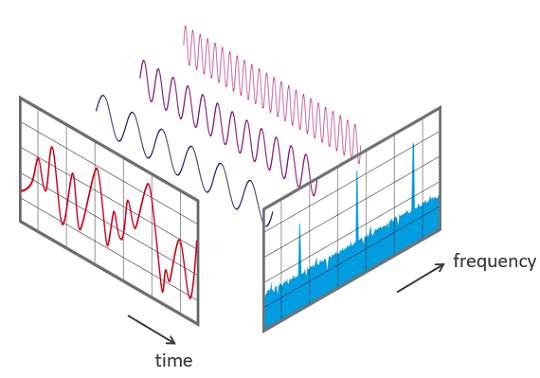
\includegraphics[width=0.5\textwidth]{imgs/fft_time_freq.png}
    \caption{Time to frequency signal decomposition \source{fftntiaudio}}
    \label{fig:signal-decomposition}
\end{figure}

% REVIEW
Since the sine and consine waves are in simple waveforms they can then be manipulated with relative ease. This process is constantly present in communications since the transmission of data over wires and radio circuits through signals and most devices nowadays perform it frequently


% TODO:
% - Elaborate more
% - Maybe describe the polynomial multiplication too
% - Maybe move the 'jia2014polynomial' citation
% . . .

And much more applications such as polynomial multiplication \cite{jia2014polynomial}, numerical integration, time-domain interpolation, x-ray diffracition ...

% \begin{tikzpicture}
%   \begin{axis}[
%       axis lines = left,
%       xlabel = \(x\),
%       ylabel = {\(f(x)\)},
%   ]
%   %Below the red parabola is defined
%   \addplot [
%       domain=-10:10, 
%       samples=100, 
%       color=red,
%   ]
%   {x^2 - 2*x - 1};
%   \addlegendentry{\(x^2 - 2x - 1\)}
%   %Here the blue parabola is defined
%   \addplot [
%       domain=-10:10, 
%       samples=100, 
%       color=blue,
%       ]
%       {x^2 + 2*x + 1};
%   \addlegendentry{\(x^2 + 2x + 1\)}
  
%   \end{axis}
%   \end{tikzpicture}
% Dar 2 exemplos principais de como é aplicado e uma breve explicação
% - Signal processing

% Denote in the end that we'll use a different case of application for this comparison (might not be true since we could use the image processing case as study)


\section{Discrete Fourier Transform} \label{sec:discrete-fourier-transform}
% \section{Discrete Fourier Transform}

The Fourier Transform of a finite sequence of equally-spaced samples of a function is the called the \textbf{Discrete Fourier Transform} (DFT), it converts a finite set of values in \textit{time} domain to \textit{frequency} domain representation. Its the most important type of transform since it deals with a discrete amount of data and has the popular algorithm in which is the center of attention of fourier transforms, which can be implemented in machines and be computed by specialized hardware.

% Forward Discrete Fourier Transform
%FIXME: This equations are replacing the reference number for the name with '\eqname'
% It must show the name AND the number
\begin{equation} \label{eq3}
    X_{k} = \sum_{n=0}^{N-1}x_{n} \cdot e^{- \frac{i 2 \pi}{N}kn} \\ %\eqname{Forward Discrete Fourier Transform} \\
\end{equation}

% Inverse Discrete Fourier Transform
%FIXME: This equations are replacing the reference number for the name with '\eqname'
% It must show the name AND the number
\begin{equation} \label{eq4}
    x_{n} = \frac{1}{N} \sum_{k=0}^{N-1}X_{k} \cdot e^{\frac{i 2 \pi}{N}kn} \\ %\eqname{Inverse Discrete Fourier Transform} \\
\end{equation}

% REVIEW (english)
Notably, the discrete version of the Fourier Transform has some obvious differences since it deals with a discrete time sequence, the first difference is that the sum covers all elements of the input values instead of integrating the infinite domain of the function, but we can also notice that the exponential, similar to the aforesaid, divides the values by \(N\) (\(N\) being the total number of elements in the sequence) due to the inability to look at frequency and time \(ft\) continuously we instead take the \(k\)'th frequency over \(n\).

We can have a more simplified expansion of this formula with:

\begin{equation*}
    X_{k} = x_{0} + x_{1}e^{\frac{i 2 \pi}{N}k} + ... + x_{N-1}e^{\frac{i 2 \pi}{N}k(N-1)} \\
\end{equation*}

% FIXME: Maybe the word i want isn't simplified because the equation is getting longer
Having this sum simplified we then only need to resolve the complex exponential, and we can do that by replacing the \(e^{\frac{i 2 \pi}{N}kn}\) by the euler formula as mentioned before to reduce the maths to a simple sum of real and imaginary numbers.

% REVIEW (math)
\begin{equation} \label{dft_reduction}
    X_{k} = x_{0} + x_{1} (\cos{b_{1}} + i\sin{b_{1}}) + ... + x_{N-1} (\cos{b_{N-1}} + i\sin{b_{N-1}}) \\
\end{equation}

\begin{equation*}
    \text{where } \\ b_{n} = \frac{ 2 \pi}{N}kn \\
\end{equation*}


Finally we'll be left with the result as a complex number

\begin{equation*}
    X_{k} = A_{k} + i B_{k}
\end{equation*}

% 1. Explicar como funciona a aplicação da DFT a uma sequência (fazer um exemplo para sinais visto que vamos ter que mencionar a frequencia de nyquist)

\paragraph{Example} \label{example1} Let us now follow an example of calculation of the DFT for a sequence \(x\) with N number of elements.

\pagestyle{empty}
% Plot the cosine wave graph with the sample values
% \begin{figure*}
%     \begin{tikzpicture}
%         \begin{axis}[width=9cm,height=4cm,
%             axis lines = center,
%             axis on top,
%             axis line style={thick},
%             ticklabel style={fill=white,font=\scriptsize, inner sep=1pt},
%             xmin=0, xmax=360,
%             ymin=-1.9, ymax=1.9,
%             % ytick={-2,-1,...,2},
%             % xtick={-2,-1,...,2},
%             legend style={draw=none,fill=white, fill opacity=0.75, 
%                           font=\scriptsize, text opacity=1, inner sep=1pt,
%                           anchor=north east, at={(1,1)}, legend columns=-1},
%             domain=0:360,
%             samples=181,
%             no marks
%                     ]
%         \addplot +[s_orange,thick] {cos(x)};
%         \legend{$\cos(x)$}
%         \end{axis}
%     \end{tikzpicture}
% \end{figure*}

\begin{equation*}
    x = 
    \begin{bmatrix}
        1 & 0.707 & 0 & -0.707 & -1 & -0.707 & 0 & 0.707\\
    \end{bmatrix}
\end{equation*}
\begin{equation*}
    N = 8
\end{equation*}

% REVIEW: Not sure about this phrase
With this sequence we now want to transform it into the frequency domain, and for that we need to apply the Discrete Fourier Transform to each element \( x_{n} \rightarrow X_{k} \), thus, for each \(k\)'th element of \(X\) we apply the DFT for every element of \(x\).

% REVIEW: Not sure if i should put intermediate steps in this apply of the DFT
\begin{equation*}
    X_{0} = 1 \cdot e^{- \frac{i 2 \pi}{8} \cdot 0 \cdot 0} \\
        + 0.707 \cdot e^{- \frac{i 2 \pi}{8} \cdot 0 \cdot 1}  \\
        + ...  \\
        + 0.707 \cdot e^{- \frac{i 2 \pi}{8} \cdot 0 \cdot 7} \\
\end{equation*}
\begin{equation*}
    = (0 + 0i)
\end{equation*}
\begin{equation*}
    X_{1} = 1 \cdot e^{- \frac{i 2 \pi}{8} \cdot 1 \cdot 0} \\
        + 0.707 \cdot e^{- \frac{i 2 \pi}{8} \cdot 1 \cdot 1}  \\
        + ...  \\
        + 0.707 \cdot e^{- \frac{i 2 \pi}{8} \cdot 1 \cdot 7} \\
\end{equation*}
\begin{equation*}
    = (4 + 0i)
\end{equation*}

\begin{equation*}
    . . .
\end{equation*}

\begin{equation*}
    X_{7} = 1 \cdot e^{- \frac{i 2 \pi}{8} \cdot 7 \cdot 0} \\
        + 0.707 \cdot e^{- \frac{i 2 \pi}{8} \cdot 7 \cdot 1}  \\
        + ...  \\
        + 0.707 \cdot e^{- \frac{i 2 \pi}{8} \cdot 7 \cdot 7} \\
\end{equation*}
\begin{equation*}
    = (4 + 0i)
\end{equation*}

% TODO: Should i do this ^ for the idft too?

And that will produce our complex-valued output in frequency domain, as simple as that.
\begin{equation*}
    X = 
    \begin{bmatrix}
        0i & 4+0i & 0i & 0i & 0i & 0i & 0i & 4+0i\\
    \end{bmatrix}
\end{equation*}


% TODO:
% [-] 1. Justify why the hz 1 isn't with just 1 since the input sequence comes from a sampled cosine wave and mention the nyquist limit (Not sure if i want to add this)
%   [-] 1.1. Talk about the properties of the magnitude and phase 
% [x] 2. Perform this calculation as a matrix dot product and that makes it better for the computer to compute
%   [1/2] 2.1 Continue previous example but now with matrix multiplication form
% [ ] 3. Algorithmic preview of the dft
% [x] 4. Last phrase that introduces the next chapter FFT

% NOTE: 2.
\subsection{Matrix multiplication} \label{subsec:matrix-multiplication}
The example shown above is done sequentially as if each frequency pin is computed individually, but there's a way to calculate the same result by using matrix multiplication \cite{rao2018transform}. Since the operations are done equally without any extra step we can group all analysing function sinusoids (\(e^{- \frac{i 2 \pi}{N} k n}\)), also refered to as twiddle factors.

% \ref{example1}

\begin{equation*}
    W = 
    \begin{bmatrix}
        \omega_{N}^{0 \cdot 0}     & \omega_{N}^{1 \cdot 0}     & \dots  & \omega_{N}^{(N-1) \cdot 0}     \\
        \omega_{N}^{0 \cdot 1}     & \omega_{N}^{1 \cdot 1}     & \dots  & \omega_{N}^{(N-1) \cdot 1}     \\
        \vdots                     & \vdots                     & \ddots & \vdots                          \\
        \omega_{N}^{0 \cdot (N-1)} & \omega_{N}^{1 \cdot (N-1)} & \dots  & \omega_{N}^{(N-1) \cdot (N-1)} \\
    \end{bmatrix} =
    \begin{bmatrix}
        1      & 1              & \dots  & 1                          \\
        1      & \omega         & \dots  & \omega^{(N-1)}             \\
        \vdots & \vdots         & \ddots & \vdots                     \\
        1      & \omega^{(N-1)} & \dots  & \omega^{(N-1) \cdot (N-1)} \\
    \end{bmatrix}
\end{equation*}
\begin{equation*}
    \text{where } \omega_{N} = e^{- \frac{i 2 \pi}{N}}
\end{equation*}

% FIXME: I dont like the way this two phrases are right now, change later
The substitution variable \(\omega\) allows us to avoid writing extensive exponents.

The symbol \(W\) represents the transformation matrix of the Discrete Fourier Transform, also called DFT matrix, and its inverse can be defined as.

\begin{equation*}
    W^{-1} = \frac{1}{N} \cdot
    \begin{bmatrix}
        1      & 1                  & \dots  & 1                              \\
        1      & \omega_{N}         & \dots  & \omega_{N}^{(N-1)}             \\
        \vdots & \vdots             & \ddots & \vdots                         \\
        1      & \omega_{N}^{(N-1)} & \dots  & \omega_{N}^{(N-1) \cdot (N-1)} \\
    \end{bmatrix}
\end{equation*}

\begin{equation*}
    \text{where } \omega_{N} = e^{- \frac{i 2 \pi}{N}} \\
\end{equation*}

By using this matrix multiplication form we can have a more efficient way to compute the DFT in hardware.  

\begin{equation*}
    X = W \cdot x \\ %\eqname{Matrix DFT} \\
\end{equation*}
\begin{equation*}
    x = W^{-1} \cdot X \\ %\eqname{Matrix IDFT} \\
\end{equation*}

Moreover we might also want to normalize the matrix by \( \sqrt{N} \) for both Matrix DFT and IDFT instead of just normalizing the IDFT by \(N\), that will make \(W\) a unitary matrix \cite{horn2012matrix}.
The advantage of using a unitary matrix is that we only need to reasign the constant substution variable \(\omega_{N}\) to be able to invert the dft, the matrix multiplication stays the same for both DFT and IDFT. 
% FIXME: This phrase isn't good in this context, is contradicting the aforesaid.
Nevertheless later we will verify that the use of sqrt function isn't desirable for the implementation of any dft.

% NOTE: 2.1.
\paragraph{Example} \label{example1.2} Continuing the example \ref{example1}, we can adapt the aplication of the DFT to the matrix multiplication form.

\begin{equation*}
    W =
    \begin{bmatrix}
        1      & 1              & \dots  & 1               \\
        1      & \omega_{8}     & \dots  & \omega_{8}^{7}  \\
        \vdots & \vdots         & \ddots & \vdots          \\
        1      & \omega_{8}^{7} & \dots  & \omega_{8}^{49} \\
    \end{bmatrix}
\end{equation*}
\begin{equation*}
    \text{where } \omega_{8} = e^{\frac{i 2 \pi}{8}}
\end{equation*}

\begin{equation*}
    X = W \cdot x = W \cdot 
    \begin{bmatrix}
        1      \\
        0.707  \\
        \vdots \\
        0.707  \\
    \end{bmatrix} =
    \begin{bmatrix}
        0      \\
        4+0i  \\
        \vdots \\
        4+0i  \\
    \end{bmatrix}
\end{equation*}


% NOTE: 3. Algorithmic preview of the dft
\hfill \break
% NOTE: 4. Last phrase that introduces the next chapter FFT
% REVIEW: (english) Usage of word conspicuous
It's conspicuous that the complexity time for each multiplication of every singular term of the sequence with the complex exponential value is \(O(N^{2})\), hence, the computation of the Discrete Fourier Transform rises exponentially as we use longer sequences. Therefore, over time new algorithms and techniques where developed to increase the performance of this transform due to its usefulness. 


\section{Fast Fourier Transform} \label{sec:fast-fourier-transform}

The Fast Fourier Transform (FFT) is a family of algorithms that effectively compute the Discrete Fourier Transform (DFT) of a sequence and its inverse. These algorihtms essentially compute the the same result as the DFT but the direct usage of the DFT formulation is too slow for its applications. Thus, FFT algorithms exploit the DFT matrix structure by employing a divide-and-conquer approach \cite{chu1999inside} to segment its application.

Over time serveral variations of the algorithms were developed to improve the performance of the DFT and many aspects were rethought in the way we apply and produce the resulting transform, in this section we'll cover at some of those variations. % and utilities. % FIXME: Here 'utilities' doesn't fit quite right but i cant find the word i want. 

% NOTE: There's a newline here since the first block of text is introducing the FFT concept, and the next paragraph is about the algorithms and what well talk about next.

% TODO:
% 1.1 Mention some of the algorithms and authors names
% 1.2 'The one well discuss now is Radix-2' and here talk about how this two main algorithms work and why its only for power of 2 cases
% Algorithms
% 2.1

% 1.1
\paragraph{}
There are many algorithms and aproaches on the FFT family such as the well known Cooley-Tukey, known for its simplicity and effectiveness to compute any sequence with size as a power of two, but also Rader's algorithm \cite{rader1968discrete} and Bluestein's algorithm \cite{bluestein1970linear} which both deal prime sized sequences, and even the Split-radix FFT \cite{yavne1968economical} that recursively expresses a DFT of length \(N\) in terms of one smaller DFT of length \(N/2\) and two smaller DFTs of length \(N/4\). 
% FIXME: 'that recursively expresses a DFT of length N in terms of one smaller DFT of length N/2 and two smaller DFTs of length N/4.' this is cited directly from https://en.wikipedia.org/wiki/Split-radix_FFT_algorithm try to rewrite later from a good source

% 1.2
The next two sections focus on the Cooley–Tukey algorithm, most specifically the radix-2 decimation-in-time (DIT) FFT and radix-2 decimation-in-frequency (DIF) FFT, which requires the input sequence to have a power of two size.

% Describe here everything that the DIT and DIF have in common

\subsection{Radix-2 Decimation-in-Time FFT} \label{subsec:radix-2-decimation-in-time-fft}

% 1. Explain the objective and what the DIT term means in the applied algorithm
% (is one of the most used)

The Radix-2 Decimation-in-Time FFT algorithm rearranges the original Discrete Fourier Transform (DFT) formula into two subtransforms, one as a sum over the even indexed elements and other as a sum over the odd indexed elements. The \autoref{eq:dit} describes this procedure with already simplified math, and hints the recursive decomposition of the DFT of size \(N/2\).

\begin{equation} \label{eq:dit}
    X_{k} = \sum_{n=0}^{\frac{N}{2}-1}x_{2n} \cdot \omega_{N/2}^{k(2n)} + \omega_{N}^{k} \sum_{n=0}^{\frac{N}{2}-1}x_{2n+1} \cdot \omega_{N/2}^{k(2n+1)} \\
\end{equation}

\begin{equation*}
    \text{where } \omega_{N} = e^{\frac{i 2 \pi}{N}}
\end{equation*}

This formulation successfully segments the full sized DFT into two \(N/2\) sized DFT's of the even and odd indexed elements where the later is multiplied by a twiddle factor \( \omega_{N}^{k} \). 
% \( X_{N} = E_{N/2} + W * O_{N/2} \)

This algorithm is a Radix-2 Decimation-in-Time in the sence that the time values are regrouped in 2 subtransforms, and the decomposition reduces the time values to the frequency domain. Since the understanding of this algorithm can be aplied recursively, the \autoref{fig:dit-fft} illustrates the basic behaviour and represents the \(N/2\) subtransforms with boxes that can be filled by the recursive application of this algorithm to produce the frequency domain sequence.


% TODO: Cite this somewhere in these two topics
% \cite{jones2014digital}

\begin{figure}[h] 
    \centering
    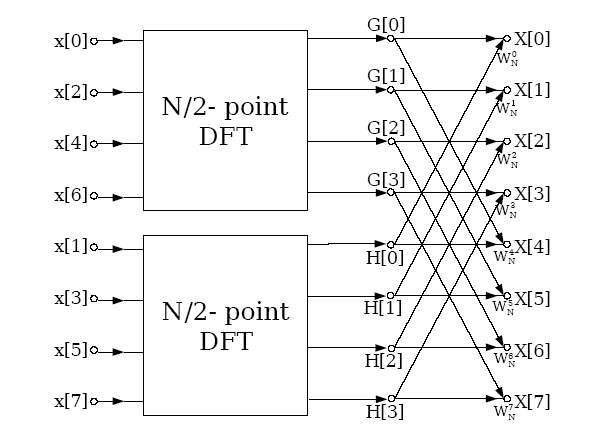
\includegraphics[width=0.5\textwidth]{imgs/dit_fft.png}
    \caption{Radix-2 Decimation-in-Time FFT \source{jones2014digital}}
    \label{fig:dit-fft}
\end{figure}

% 2. Continue explaining this algorithm

Effectivelly, this smaller DFT's are recursively reduced by this algorithm until theres only the computation of a length-2 DFT where its only applied the Cooley-Tukey butterfly operation \cite{chu1999inside} illustrated in \autoref{fig:dit-butterfly}.

% NOTE: Handmade since there wan't one that had exacly what i wanted
\begin{figure}[h] 
    \centering
    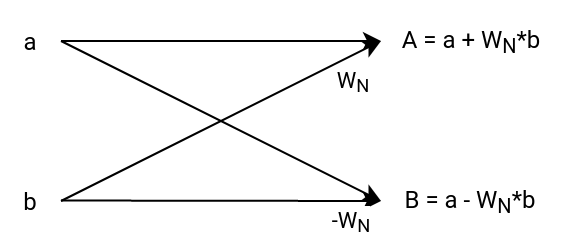
\includegraphics[width=0.5\textwidth]{imgs/dit_butterfly.png}
    \caption{Cooley-Tukey butterfly}
    \label{fig:dit-butterfly}
\end{figure}

% "Whereas direct computation of all N DFT frequencies according to the DFT equation would require N2 complex multiplies and N2−N complex additions (for complex-valued data), by reusing the results of the two short-length DFTs as illustrated in Figure, the computational cost is now" 

The complexity work within the algorithm is distributed with the DIT approach which decomposes each DFT by 2 having \(\log{N}\) stages \cite{smith2007mathematics} while there are approximately \(N\) complex multiplications needed for each stage of the DIT decomposition, therefore the multiplication complexity for a \(N\) sized DFT is reduced from \(O(N^{2})\) to \(O(N \log{N})\) without any programming specific optimizations.

In practice, \autoref{alg:dit} demonstrates the aforesaid with an iterative representation of a possible implementation. Although this algorithm is congruent with a code implementation, its worth noting that the input sequence can either have real or complex numbers, since the arithmetic is the same for both domains the only thing that needs to be specialized is the operator overloading in the inner most loop.

% 3. Algorithmic overview
\SetKwComment{Comment}{/* }{ */}
\RestyleAlgo{ruled}
\begin{algorithm}[H]
    \caption{Radix-2 Decimation-in-Time Forward FFT} \label{alg:dit}
    \KwData{Sequence $in$ with size $N$ power of 2 }
    \KwResult{Sequence $out$ with size $N$ with the DFT of the input}

    \Comment{Bit reversal step}
    \ForEach{$i = 0$ \textbf{to} $N-1$}{
        $out[$bit\_reverse$(i)] \gets in[i]$
    }

    \Comment{FFT}
    \ForEach{$s = 1$ \textbf{to} $\log{N} $}{
        $m \gets 2^{s}$\;
        $w_{m} \gets \exp(-2\pi i / m)$\;
        \ForEach{$k = 0$ \textbf{to} $N-1$ \textbf{by} $m$}{
            $w \gets 1$\;
            \ForEach{$j = 0$ \textbf{to} $m/2$}{
                $bw \gets w \cdot out[k + j + m/2] $\;
                $a \gets out[k + j] $\;
                $out[k + j] \gets a + bw$\;
                $out[k + j + m/2] \gets a - bw$\;
                $w \gets w \cdot w_{m}$\;
            }
        }
    }
    \textbf{return} $out$\;
\end{algorithm}

\subsection{Radix-2 Decimation-in-Frequency FFT} \label{subsec:radix-2-decimation-in-frequency-fft}

% 1. Explain the objective and what the DIF term means in the applied algorithm
The Radix-2 Decimation-in-Frequency FFT algorithm is very similar to the DIT approach, its based on the same principle of divide-and-conquer but it rearranges the original Discrete Fourier Transform (DFT) into the computation of two transforms, one with the even indexed elements and other with the odd indexed elements; as in this simplified formulation \autoref{eq:dif}.

\begin{equation} \label{eq:dif}
    \begin{aligned}
        X_{2k} &= \sum_{n=0}^{\frac{N}{2}-1} (x_{n} + x_{n + \frac{N}{2}}) \cdot \omega_{N/2}^{kn} \\
        X_{2k+1} &= \sum_{n=0}^{\frac{N}{2}-1} ((x_{n} - x_{n + \frac{N}{2}}) \cdot \omega_{N/2}^{kn}) \cdot \omega_{N}^{n} \\
    \end{aligned}
\end{equation}

\begin{equation*}
    \text{where } \omega_{N} = e^{\frac{i 2 \pi}{N}}
\end{equation*}

The DFT divided into these two transforms from the full sized DFT
By separating these two transforms from the full sized DFT we get two distinct 

Notably, this formulation distinguishes the full sized DFT into two \(N/2\) sized DFT's of the even and odd indexed elements where the later is multiplied by a twiddle factor \( \omega_{N}^{k} \) with both outside the same context. 
% \( X_{N} = E_{N/2} + W * O_{N/2} \)

This algorithm is a Radix-2 Decimation-in-Frequency since the DFT is deciminated into two distinct smaller DFT's and the frequency samples will be computed separately in different groups, as if the regrouping of the DFT's would reduce directly to the frequency domain. Since the understanding of this algorithm can be aplied recursively, the \autoref{fig:dif-fft} illustrates the this behaviour and represents the \(N/2\) subtransforms with boxes that can be filled by the recursive application of this algorithm to produce the frequency domain sequence. Aditionally this illustration can be compared to \autoref{fig:dit-fft} since both are symmetrically identical.

\begin{figure}[h] 
    \centering
    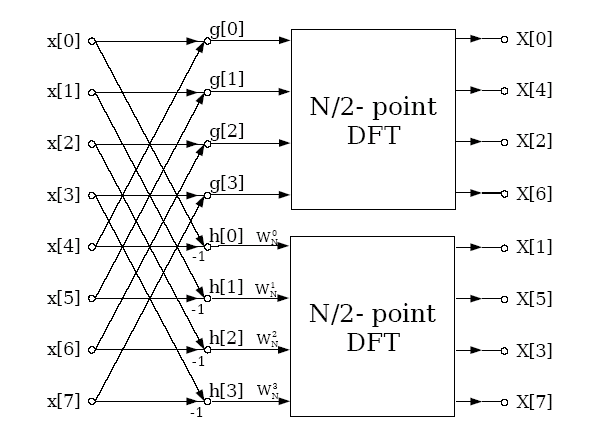
\includegraphics[width=0.5\textwidth]{imgs/dif_fft.png}
    \caption{Radix-2 Decimation-in-Frequency FFT \source{jones2014digital}}
    \label{fig:dif-fft}
\end{figure}

Similarly to the DIT version, the DFT can be recursively reduced by the DIF algorithm until theres only the computation of a length-2 DFT where its only applied the Gentleman-Sande butterfly operation \cite{chu1999inside} illustrated in \autoref{fig:dif-butterfly}.

% NOTE: Handmade since there wan't one that had exacly what i wanted
\begin{figure}[h]
    \centering
    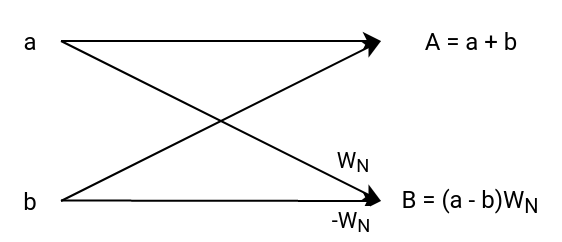
\includegraphics[width=0.5\textwidth]{imgs/dif_butterfly.png}
    \caption{Gentleman-Sande butterfly}
    \label{fig:dif-butterfly}
\end{figure}

Since this algorithm has similarities with the DIT, its complexity also lives to this similarity, maintaining the same \(O(N \log{N})\) for number of multiplications, despite that, \autoref{fig:dif-butterfly} and \autoref{fig:dit-butterfly} might look different in number of arithmetic operations since the first has 1 addition, 1 subtraction, and 2 multiplications, and the second has 1 addition, 1 subtraction, and 1 multiplication, but effectively the \(W_{N} \cdot b\) can be reused and only computed once as seen in \autoref{alg:dit}.
% FIXME: The complexity work within the algorithm is distributed with the DIT approach which decomposes each DFT by 2 having \(\log{N}\) stages \cite{smith2007mathematics} while there are approximately \(N\) complex multiplications needed for each stage of the DIT decomposition, therefore the multiplication complexity for a \(N\) sized DFT is reduced from \(O(N^{2})\) to \(O(N \log{N})\) without any programming specific optimizations.


% FIXME: im repeating exactly whats in the DIT but its exactly what i want to say, what to do? keep this or change?
In practice, \autoref{alg:dif} demonstrates the aforesaid with an iterative representation of a possible implementation. Although this algorithm is congruent with a code implementation, its worth noting that the input sequence can either have real or complex numbers, since the arithmetic is the same for both domains the only thing that needs to be specialized is the operator overloading in the inner most loop.

% 3. Algorithmic overview
\SetKwComment{Comment}{/* }{ */}
\RestyleAlgo{ruled}
\begin{algorithm}[H]
    \caption{Radix-2 Decimation-in-Frequency Forward FFT} \label{alg:dif}
    \KwData{Sequence $in$ with size $N$ power of 2 }
    \KwResult{Sequence $out$ with size $N$ with the DFT of the input}

    \Comment{FFT}
    \ForEach{$s = 0$ \textbf{to} $\log{N}-1 $}{
        $gs \gets N \gg s$\;
        $w_{gs} \gets \exp(2\pi i / gs)$\;
        \ForEach{$k = 0$ \textbf{to} $N-1$ \textbf{by} $gs$}{
            $w \gets 1$\;
            \ForEach{$j = 0$ \textbf{to} $gs/2$}{
                $a \gets in[k + j + gs/2] $\;
                $b \gets in[k + j] $\;
                $in[k + j] \gets a + b$\;
                $in[k + j + gs/2] \gets (a - b) \cdot w$\;
                $w \gets w \cdot w_{gs}$\;
            }
        }
    }
    
    \Comment{Bit reversal step}
    \ForEach{$i = 0$ \textbf{to} $N-1$}{
        $out[$bit\_reverse$(i)] \gets in[i]$
    }

    \textbf{return} $out$\;
\end{algorithm}



% % Algorithms side by side
% \begin{figure}[!ht]
%     \centering
%     \begin{subfigure}{.45\textwidth}
%         \centering
%         % Alg 1
%         \caption{Test Algorithm No.1}\label{alg:alg-1}
%     \end{subfigure}

%     \hfill

%     \begin{subfigure}{.45\textwidth}
%         \centering
%         % Alg 2
%         \caption{Test Algorithm No.2}\label{alg:alg-2}
%     \end{subfigure}
% \end{figure}


% \subsection{2D and 3D transforms}

% Altough we've already gonne through a lot of information ... its still unclear how these primitive functions on multidimentional targets, such as images.

% % TODO:
% Empty


% \section{Related Work}

% %TODO: 
% Empty

% \subsection{cuFFT}

% %TODO: 
% Empty

% \subsection{Fast Computation of general Fourier Transforms on GPUS}

% %TODO: 
% Empty
% Talk about that microsoft paper which implements efficiently in HLSL

%%%%%%%%%%%%%%%%%%%%%%%%%%%%%%%%%%%%%%%%%%%%%%%%%%%%%%%%%%%%%%%%
%                     Algorithms analysis                      %
%%%%%%%%%%%%%%%%%%%%%%%%%%%%%%%%%%%%%%%%%%%%%%%%%%%%%%%%%%%%%%%%
\chapter{Algorithms analysis}


To flavour this pre-dissertation report some work of benchmarking and analysis were done to compete with the theoretical explanations addressed on \autoref{chap:state-of-the-art}. Hence, some implementations were tested to provide coherence to what has been studied, and algorithms such as \autoref{alg:dit} Radix-2 Decimantion-in-Time \autoref{alg:dif} Radix-2 Decimantion-in-Frequency were timed in \autoref{tab:benchmarking}.

\begin{table}[h]
    \centering
    \normalsize
    \sffamily
    \renewcommand{\arraystretch}{1.5}%
    \begin{tabular}{|c|l|l|l|l|l|}
        \hline
        \multicolumn{1}{|l|}{} & \multicolumn{1}{c|}{\textbf{Size 128}} & \multicolumn{1}{c|}{\textbf{Size 256}} & \multicolumn{1}{c|}{\textbf{Size 512}} & \multicolumn{1}{c|}{\textbf{Size 1024}} & \multicolumn{1}{c|}{\textbf{Size 2048}} \\ \hline
        \textbf{DFT}           & 5.16593                                & 17.2782                                & 70.5689                                & 293.104                                 & 1246.44                                 \\ \hline
        \textbf{FFT  DIT}      & 0.169113                               & 0.37668                                & 0.86415                                & 1.8793                                  & 4.47742                                 \\ \hline
        \textbf{FFT DIF}       & 0.159458                               & 0.378722                               & 0.881921                               & 1.90661                                 & 4.13369                                 \\ \hline
        \textbf{Recursive FFT} & 0.210895                               & 0.485643                               & 1.4421                                 & 2.32922                                 & 5.1178                                  \\ \hline
    \end{tabular}
    \caption{FFT algorithms benchmark. Results are \underline{measured in milliseconds} for forward and inverse computation with varying input sizes}
    \label{tab:benchmarking}
\end{table}

As we can see the Discrete Fourier Transform increases exponentially for higher sized sequences, as expected all FFT variants perform critically better than the original formulation.

One variant that wasn't exposed much in the above chapters is the Recursive FFT algorithm, which corresponds to a Decimation-in-Time aproach with recursive reduction, therefore this algorithm aggregates the divide-and-conquer method but with the disadvantage of recursive function overhead. This recursive look at the DIT approach can be easier to implement since the bit reversal step isn't explicitly applied before starting the FFT.

Finally, as expected the DIT and DIF algorithms overrule the other alternatives for every sized input.

% (DIT FFT) (DIF FFT) DFT
% (DIT FFT no bit reversal) (DIF FFT no bit reversal) DFT
% (FFT Recursive) DFT


%%%%%%%%%%%%%%%%%%%%%%%%%%%%%%%%%%%%%%%%%%%%%%%%%%%%%%%%%%%%%%%%
%             Computation of the Fourier Transform             %
%%%%%%%%%%%%%%%%%%%%%%%%%%%%%%%%%%%%%%%%%%%%%%%%%%%%%%%%%%%%%%%%
\chapter{Computation of the Fourier Transform}


\section{Improving the Cooley-Tukey algorithm}
Nowadays there is a lot more to the computation of FFT's than just the basic Cooley-Tukey algorithm described in \ref{subsec:radix-2-decimation-in-time-fft} there are more algorithms, variations and improvements that enhace the computation in many aspects. Even the target hardware can change the restrictions on the computation of this primitive.

One could optimize the fft by providing precomputed twiddle factors, or spare space for the output sequence by adopting an inplace FFT algorithm  and all those factors influence the performance, evidently a balance must be stablished depending on the constraints for the FFT.

\subsection{Natural order Cooley-Tukey}


\subsection{Stockham algorithm}
\subsection{Radix-4 instead of Radix-2}


%%%%%%%%%%%%%%%%%%%%%%%%%%%%%%%%%%%%%%%%%%%%%%%%%%%%%%%%%%%%%%%%
%                  Implementation on the GPU                   %
%%%%%%%%%%%%%%%%%%%%%%%%%%%%%%%%%%%%%%%%%%%%%%%%%%%%%%%%%%%%%%%%
\chapter{Implementation on the GPU}
\section{Fourier Transform on the GPU}
\section{Implementation in GLSL}

%%%%%%%%%%%%%%%%%%%%%%%%%%%%%%%%%%%%%%%%%%%%%%%%%%%%%%%%%%%%%%%%
%                   Analysis and Comparison                    %
%%%%%%%%%%%%%%%%%%%%%%%%%%%%%%%%%%%%%%%%%%%%%%%%%%%%%%%%%%%%%%%%
\chapter{Analysis and Comparison}
\section{Popular implementations}
\subsection{cuFFT}
\subsection{FFTW}
\section{Comparison with GLSL implementation}
\subsection{Analysis}
Popular implementations

%%%%%%%%%%%%%%%%%%%%%%%%%%%%%%%%%%%%%%%%%%%%%%%%%%%%%%%%%%%%%%%%
%                     END OF MAIN CHAPTERS                     %
%%%%%%%%%%%%%%%%%%%%%%%%%%%%%%%%%%%%%%%%%%%%%%%%%%%%%%%%%%%%%%%%

\bookmarksetup{startatroot} % Ends last part.
% \addtocontents{toc}{\bigskip} % Making the table of contents look good.
\cleardoublepage

% Bibliography (requires 'bibtex'  package)
\addcontentsline{toc}{chapter}{Bibliography}
\bibliographystyle{acm}
\bibliography{dissertation}
% Index of terms (required 'makeindex' package)
\printindex

    
    \appendix
    \renewcommand\chaptername{Appendix}

    % Add appendix chapters

%%%%%%%%%%%%%%%%%%%%%%%%%%%%%%%%%%%%%%%%%%%%%%%%%%%%%%%%%%%%%%%%%

% \part{Appendices}

%%%%%%%%%%%%%%%%%%%%%%%%%%%%%%%%%%%%%%%%%%%%%%%%%%%%%%%%%%%%%%%%%

% \chapter{Support work}
% 	Auxiliary results which are not main-stream

%%%%%%%%%%%%%%%%%%%%%%%%%%%%%%%%%%%%%%%%%%%%%%%%%%%%%%%%%%%%%%%%%

% \chapter{Details of results}
%          Details of results whose length would compromise readability of main text.

%%%%%%%%%%%%%%%%%%%%%%%%%%%%%%%%%%%%%%%%%%%%%%%%%%%%%%%%%%%%%%%%%

% \chapter{Listings}
% 	Should this be the case

%%%%%%%%%%%%%%%%%%%%%%%%%%%%%%%%%%%%%%%%%%%%%%%%%%%%%%%%%%%%%%%%%

% \chapter{Tooling}
% 	(Should this be the case)

% 	Anyone using \Latex\ should consider having a look at \TUG,
% 	the \tug{\TeX\ Users Group}

%%%%%%%%%%%%%%%%%%%%%%%%%%%%%%%%%%%%%%%%%%%%%%%%%%%%%%%%%%%%%%%%%

% \begin{backcover}
% \thispagestyle{empty} \pagecolor{white} \textcolor{black} {\fontfamily{phv}\fontseries{mc}\selectfont ~\vfill
% \noindent
% NB: place here information about funding, FCT project, etc in which the work is framed. Leave empty otherwise.
% %
% \vfill ~}
% \end{backcover}

\end{document}
